\subsection{algorithmic analyse-and-refactor actions  on Stream Topologies}\label{algo}

This section elaborates on the algorithmic analyse-and-refactor actions  supported by OSTIA using the common graph-like notation introduced previously. OSTIA currently supports two topology content analysis (see Sec. \ref{1} and \ref{2}) as well as two topology layout analyses (see Sec. \ref{3} and \ref{4}). Only a part of these analyses is currently implemented in OSTIA. We discuss approach limitations further in Sect. \ref{disc}.\todoMB{}{Frase critica critica da rev. Solo alcune sono implementate.}

\subsubsection{Fan-in/Fan-out}\label{1}

The Fan-in/Fan-out algorithmic analyse-and-refactor action is outlined in Fig. \ref{fig:fan}. For each element of the topology, fan-in is the number of incoming
streams. Conversely, fan-out is the number outgoing streams. In the case of
bolts, both in and out streams are internal to the topology. For Spouts,
incoming streams are the data sources of the topology (e.g., message brokers,
APIs, etc) which live outside of the topology.

\begin{figure}
	\begin{center}
		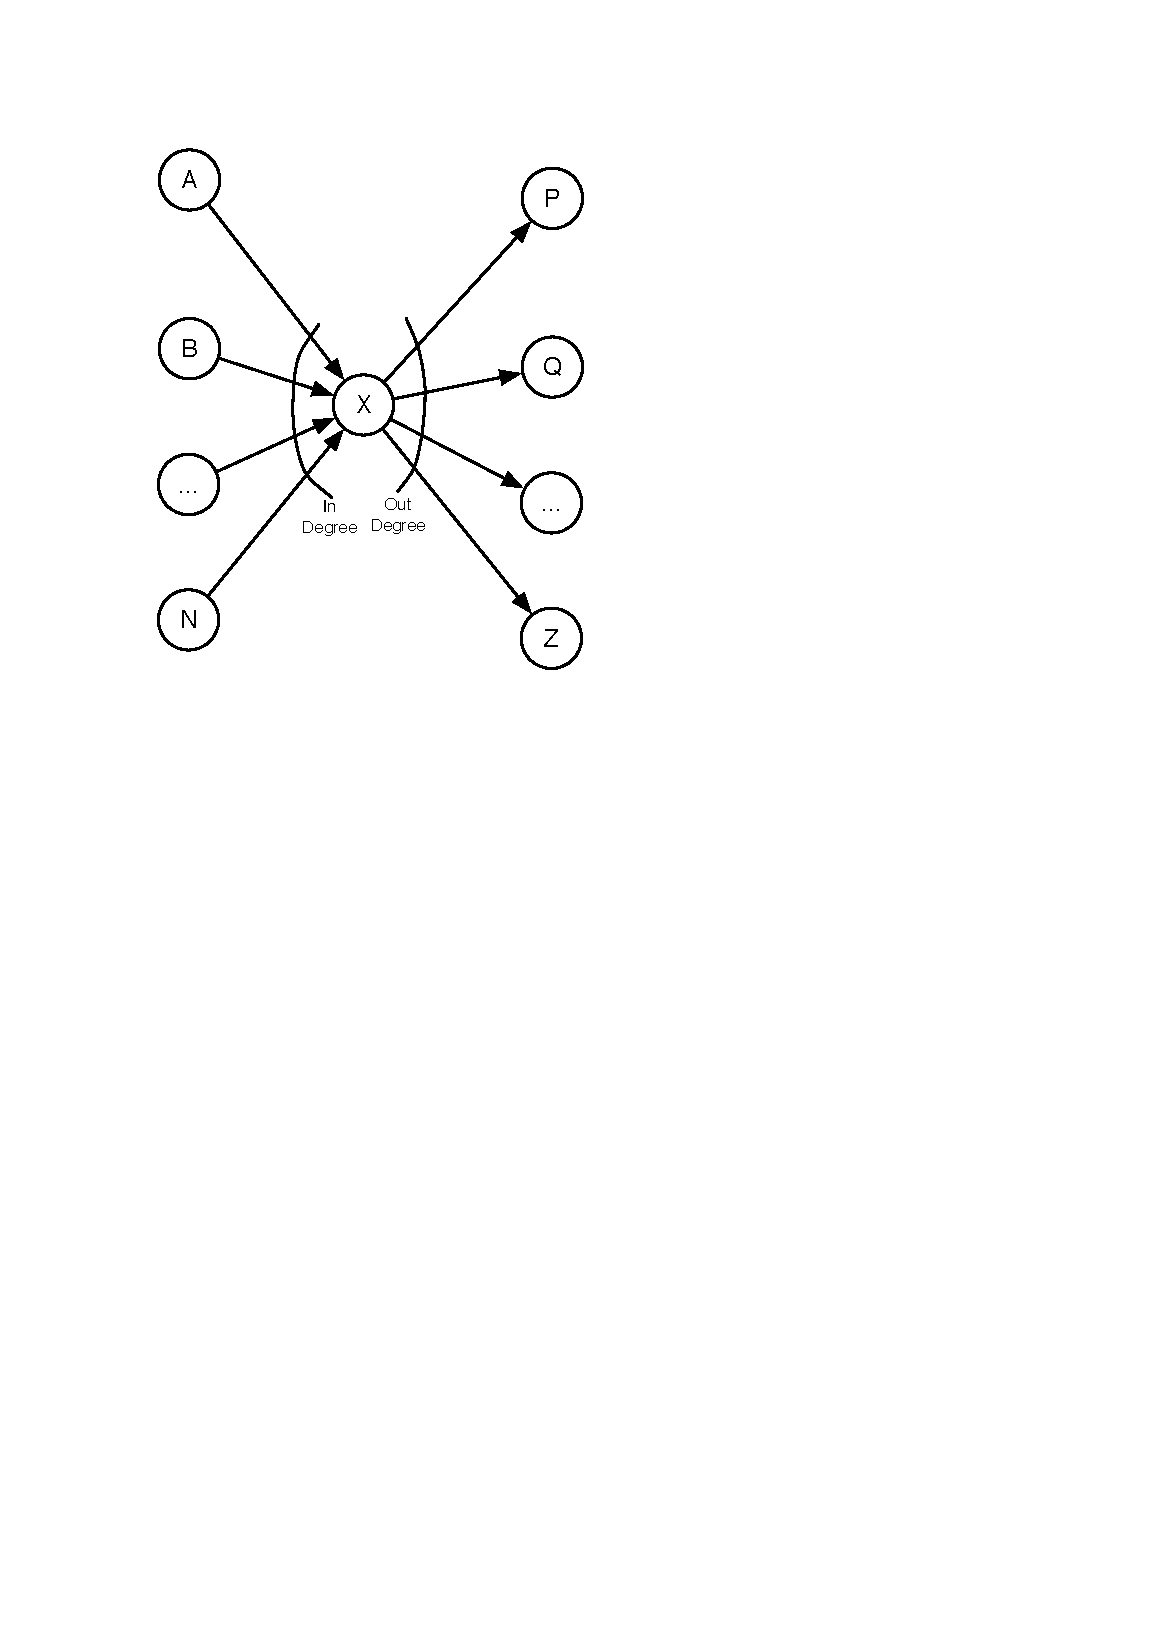
\includegraphics[width=3cm]{images/fan-in-out}
		\caption{Fan-in fan-out in Stream topologies.}
		\label{fig:fan}
	\end{center}
\end{figure}

This algorithmic analyse-and-refactor action allows to visualise instances where fan-in and fan-out numbers are differing.\todoMB{}{Solo visual quindi.}

\subsubsection{Topology cascading}\label{2}

The Cascading algorithmic analyse-and-refactor action is outlined in Fig. \ref{fig:cascading}. By topology cascading, we mean connecting two different Storm topologies via a messaging framework (e.g., Apache Kafka~\cite{kafka}).
%\footnote{\url{http://kafka.apache.org/}}). 
Although cascading may simplify the development of topologies by encouraging architecture elements' reuse especially for complex but procedural topologies, this circumstance may well raise the complexity of continuous architecting and may require separation of concerns \cite{soc}. For example, Fig. \ref{fig:cascading} outlines an instance in which two topologies are concatenated together by a message broker. In this instance, formal verification may be applied on the left-hand side topology, which is more business-critical, while the right-hand side of the entire topology is improved by on-the-fly OSTIA-based analysis. Even though OSTIA support for this feature is still limited, we report it nonetheless since OSTIA was engineered to address multiple topologies at once. 
%More details on this and similar limitations are discussed in Section \ref{lim}.
%\emph{\bf Ostia does not support this. I can't think of an easy way to implement it}

\begin{figure}
	\begin{center}
		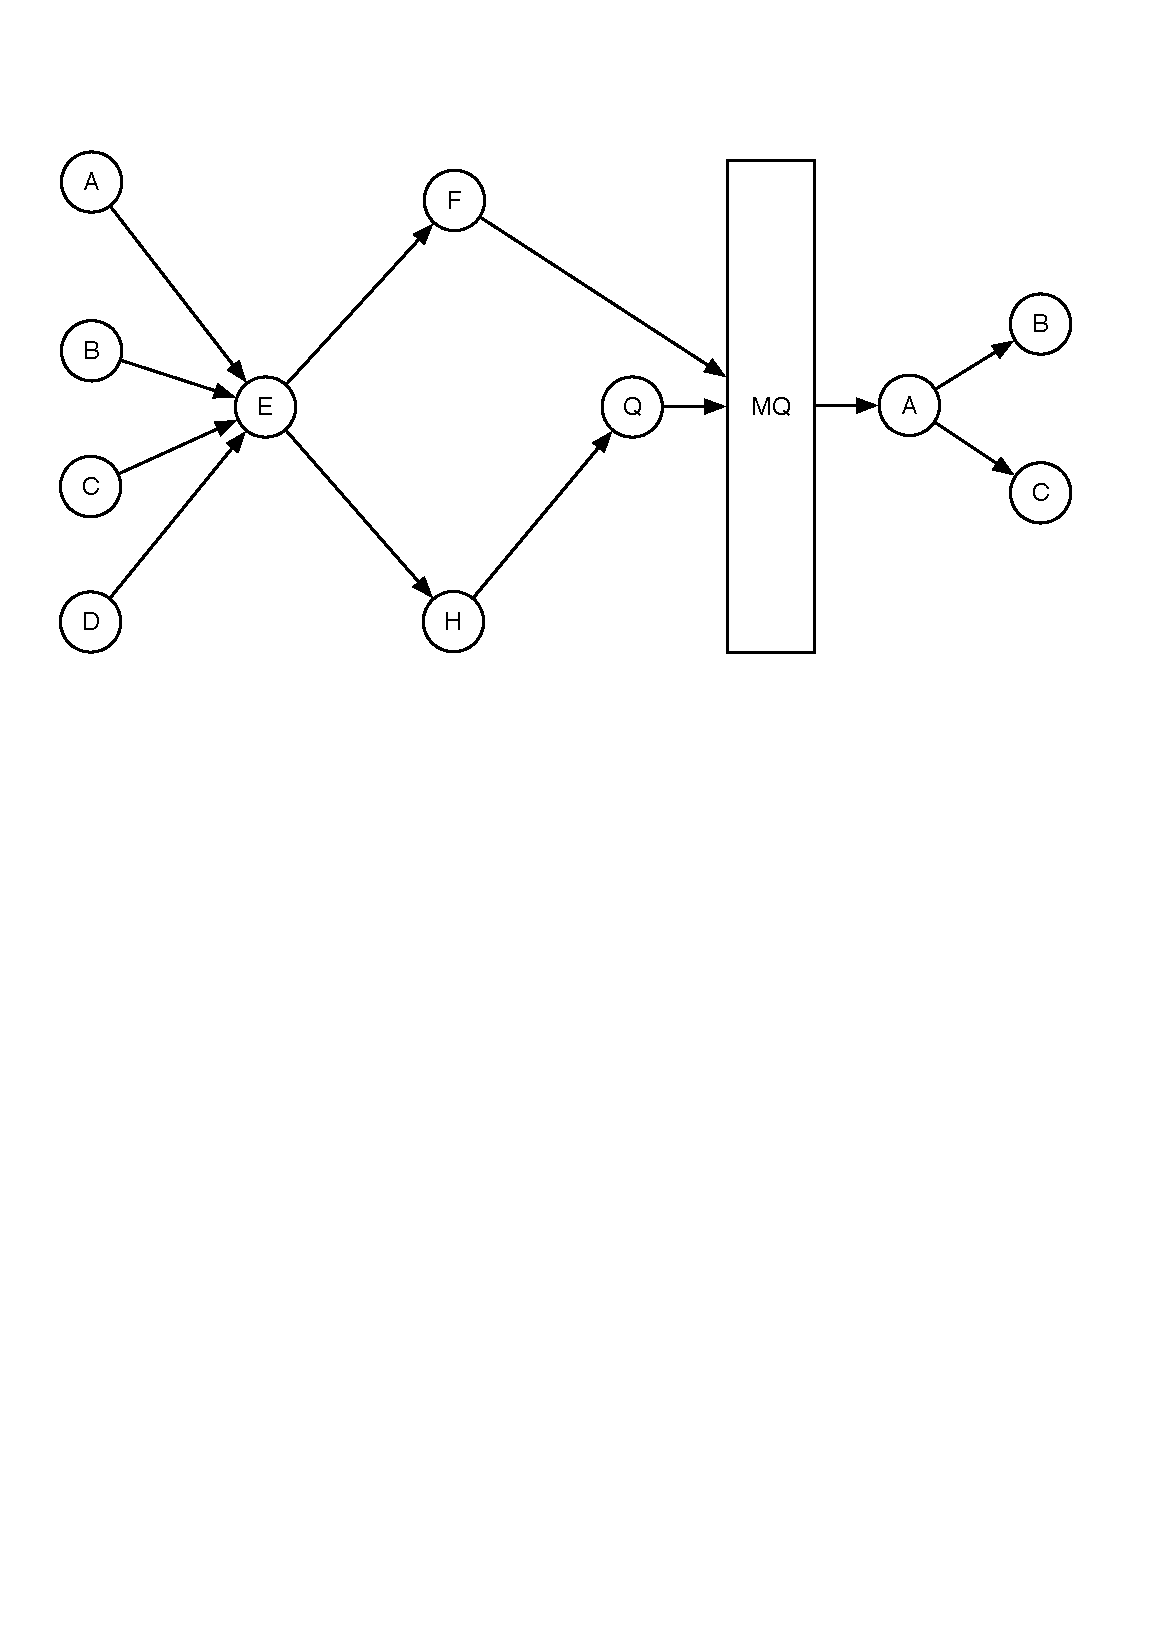
\includegraphics[width=6cm]{images/cascading}
		\caption{cascading.}
		\label{fig:cascading}
	\end{center}
\end{figure}

This algorithmic action allows to combine multiple cascading topologies.\todoMB{}{Non mi e' chiaro cosa faccia questa azione? E' visuale?}


\subsubsection{Topology clustering}\label{3}
Topology clustering is outlined in Fig. \ref{fig:clustering}. Topology clustering implies identifying coupled processing elements (i.e., bolts and spouts) and cluster them together (e.g., by means of graph-based analysis) in a way that elements in a cluster have high cohesion and loose-coupling with elements in other clusters. Simple clustering or Social-Network Analysis mechanisms can be used to infer clusters. These clusters may require additional attention since they could turn out to become bottlenecks. Reasoning more deeply on clusters and their resolution may lead to establishing the Storm scheduling policy best-fitting with the application. We will elaborate on this in Section \ref{sec:performance-boosting}.
%\emph{\bf Does it relates with Storm scheduling?}

\begin{figure}
	\begin{center}
		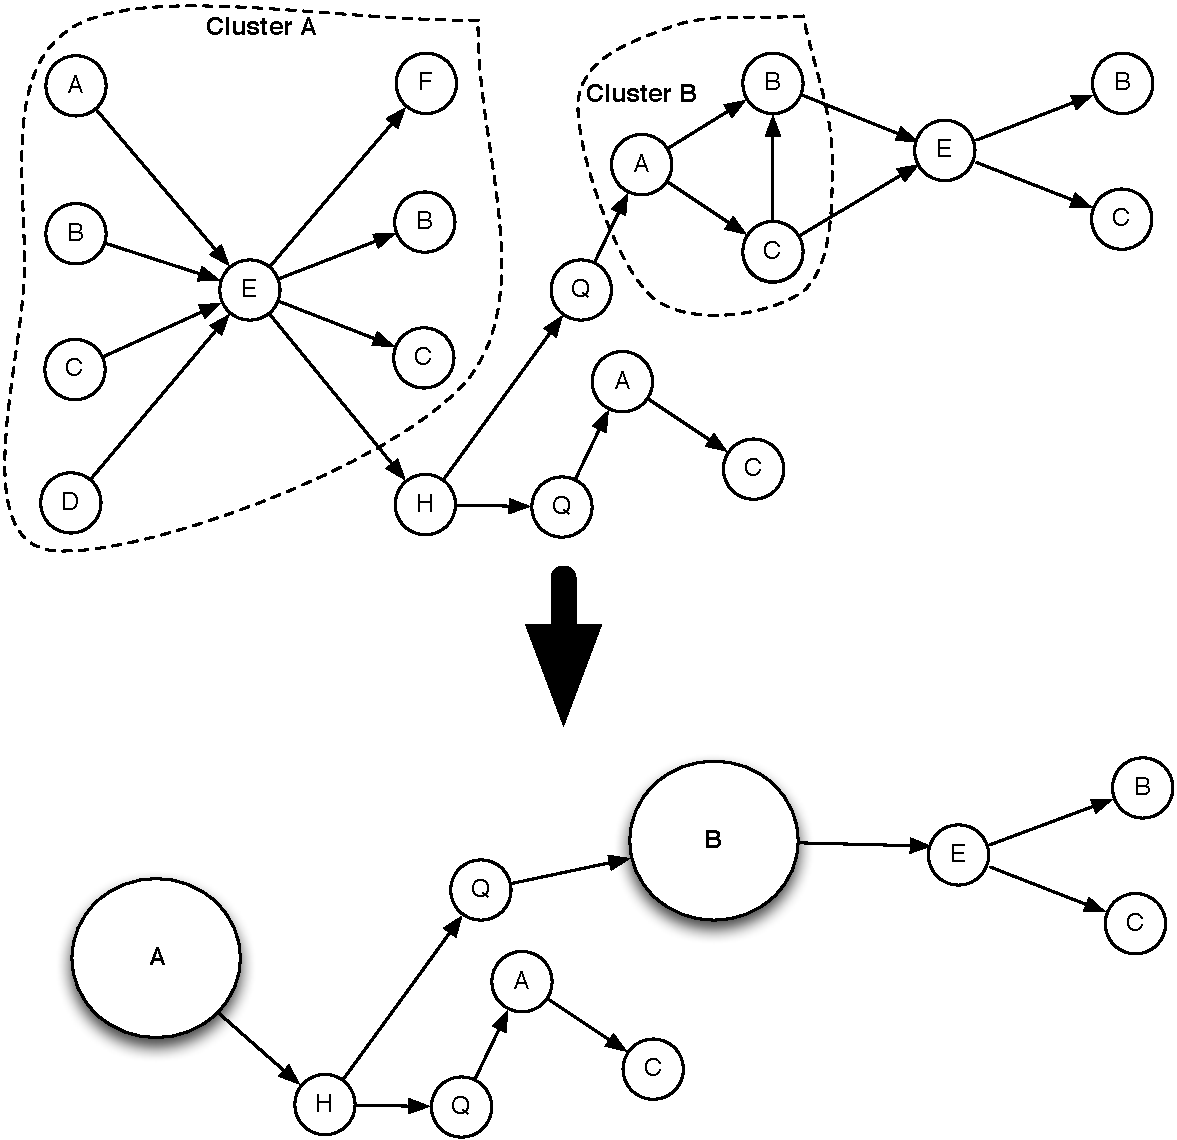
\includegraphics[width=6.5cm]{images/clustering}
		\caption{clustering.}
		\label{fig:clustering}
	\end{center}
\end{figure}


\subsubsection{Linearising a topology}\label{4}

Topology linearisation is outlined in Fig. \ref{fig:linearizing}. Sorting the processing elements in a topology in a way that topology looks more linear, visually. This step ensures that visual investigation and evaluation of the structural complexity of the topology is possible by direct observation. It is sometimes essential to provide such a visualisation to evaluate how to refactor the topology as needed.

\begin{figure}
	\begin{center}
		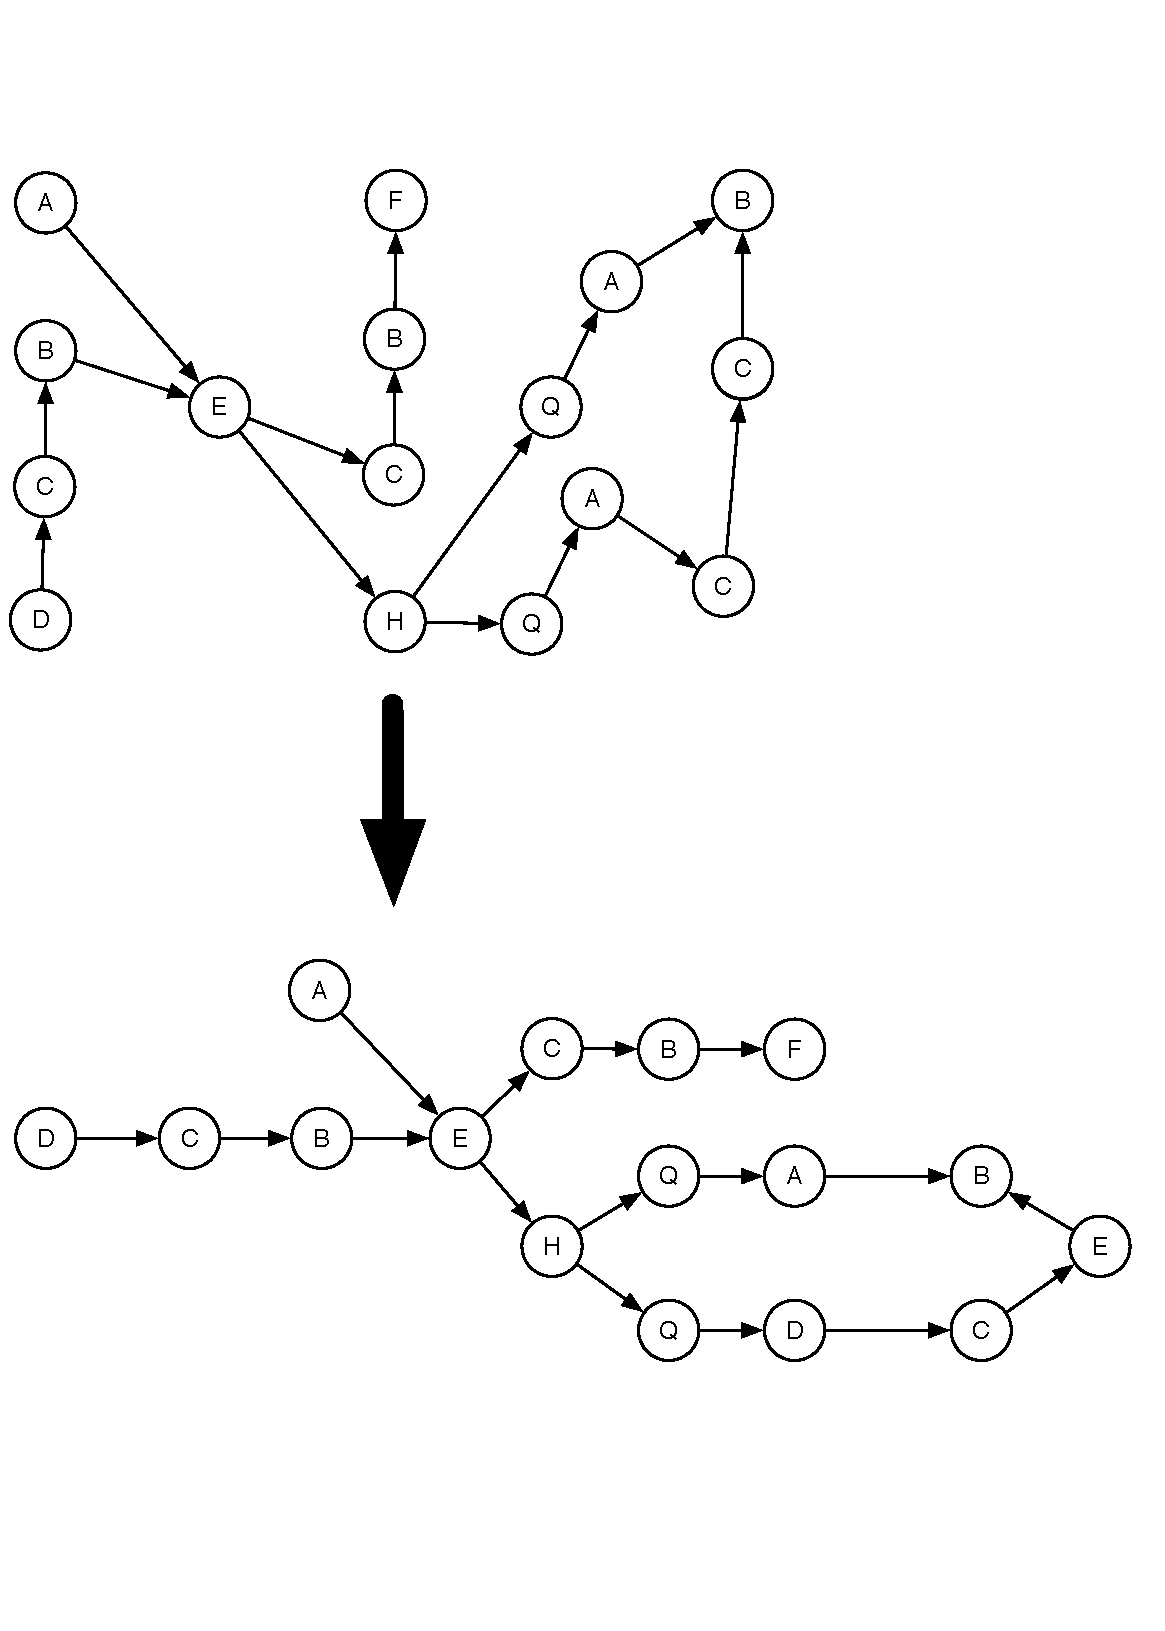
\includegraphics[width=5cm]{images/linearizing}
		\caption{linearising.}
		\label{fig:linearizing}
	\end{center}
\end{figure}